\documentclass[sigconf]{acmart}
% Cleaning
\pagestyle{fancy} % removes running headers
\settopmatter{printacmref=false} % Removes citation information below abstract
\renewcommand\footnotetextcopyrightpermission[1]{} % removes footnote with conference information in first column
\pagestyle{plain} % removes running headers
\fancyhead{}
\settopmatter{printacmref=false, printfolios=false}
% Copyright
\setcopyright{none}
\settopmatter{printacmref=false} % Removes citation information below abstract
\acmDOI{}

\usepackage{booktabs} % For formal tables
\usepackage{url}
\usepackage{algorithm}
\usepackage[noend]{algpseudocode}
\algtext*{EndWhile}% Remove "end while" text
\algtext*{EndIf}% Remove "end if" text
\algtext*{EndFor}% Remove "end for" text

\setlength{\parskip}{0pt}
\setlength{\parsep}{0pt}
\setlength{\headsep}{0pt}
\setlength{\topskip}{0pt}
\setlength{\topmargin}{0pt}
\setlength{\topsep}{0pt}
\setlength{\partopsep}{0pt}
\usepackage{mdwlist}
\usepackage{amsmath}
\usepackage{tikz}
\usetikzlibrary{positioning,arrows.meta,fit}

\begin{document}
\title{Learning USV Drift from Telemetry: Linear, LSTM and Transformer Models}
\author{Jake Cushway}
\affiliation{
  \institution{University of Victoria}
  \city{Victoria}
  \country{Canada}
}
\email{jakecush1@uvic.ca}

\author{Rowan Hall}
\affiliation{
  \institution{University of Victoria}
  \city{Victoria}
  \country{Canada}
}
\email{rowanhall@uvic.ca}

\begin{abstract}
A shore pilot keeps the Open Ocean Robotics DataXplorer\texttrademark{} USV within 10~nm of a retired NOAA buoy, letting it drift with the motor off and correcting it before it nears the boundary. Knowing where the vessel will be in an hour is the first step toward predicting \emph{when} the pilot must act. We formalise drift prediction as regression from the last 60~minutes of telemetry (position and wind) to the displacement over the next 60~minutes, and compare a persistence baseline, linear regression, an LSTM and a transformer under a deployment-wise split. Code: \url{https://github.com/jakecush1/autonomous-pilot-ML} (\texttt{usv-intervention/v1\_ml/rowan}).\footnote{AI use (Guideline D): the code and a first draft of this paper were generated with Claude (Anthropic) and reviewed, run and edited by the authors.}
\end{abstract}

\keywords{Uncrewed surface vehicle, drift prediction, time series regression, LSTM, transformer}
\maketitle
\pagestyle{empty}

\section{Problem Definition}\label{sec:problem}
Let a deployment be a 1-minute telemetry sequence $\mathcal{S}=\{s_\tau\}_{\tau=1}^{T}$ with $s_\tau=(\phi_\tau,\lambda_\tau,v_\tau,\theta_\tau,m_\tau)$: latitude, longitude, wind speed (kn), the compass direction the wind blows \emph{from}, and motor power (W). A minute is \emph{drifting} if $m_\tau=0$. Given a time $t$ at which the vessel has drifted for the past $H$ minutes, we want a function
\begin{equation}\label{eq:f}
f:\mathbb{R}^{H\times 4}\rightarrow\mathbb{R}^{2},\qquad \hat{\mathbf{y}}_t=f(\mathbf{X}_t),
\end{equation}
where $\mathbf{X}_t$ is the past window (\S\ref{sec:repr}) and $\mathbf{y}_t=\mathbf{p}_{t+H}-\mathbf{p}_t\in\mathbb{R}^2$ is the east/north displacement in metres over the next $H$ minutes, assuming the motor stays off. The predicted position is $\hat{\mathbf{p}}_{t+H}=\mathbf{p}_t+\hat{\mathbf{y}}_t$. This is regression, not classification: the output is a continuous vector. We use $H=60$.

\section{Proposed Approach}\label{sec:approach}
\subsection{Representation}\label{sec:repr}
\textbf{Position.} Each fix is projected to metres east/north of the station centre $(\phi_0,\lambda_0)$ with an equirectangular projection, with $<0.3\%$ distance error within 10~nm: $\mathbf{p}_\tau=R\,\big((\lambda_\tau-\lambda_0)\cos\phi_0,\;\phi_\tau-\phi_0\big)$, $R=6371$\,km, angles in radians.
\textbf{Wind.} Direction is averaged as $(\sin\theta,\cos\theta)$ so it is continuous across north. The wind pushes the vessel the opposite way, so the push vector is $\mathbf{w}_\tau=-v_\tau(\sin\theta_\tau,\cos\theta_\tau)$ (east, north).
\textbf{Window.} With $\Delta\mathbf{p}_\tau=\mathbf{p}_\tau-\mathbf{p}_{\tau-1}$, the input is the sequence
$\mathbf{X}_t=[\,(\Delta\mathbf{p}_\tau,\mathbf{w}_\tau)\,]_{\tau=t-H+1}^{t}\in\mathbb{R}^{H\times4}$.

\subsection{Preprocessing and Sample Selection}
Gaps of $\leq5$ missing minutes are linearly interpolated (motor power is forward-filled). A minute is \emph{valid} if $m_\tau=0$, all features exist, and $\|\Delta\mathbf{p}_\tau\|<93$\,m (about 3\,kn; faster means towing or transit, not drift). Time $t$ yields a sample $(\mathbf{X}_t,\mathbf{y}_t)$ only if all $2H$ minutes $t-H+1,\dots,t+H$ are valid, so neither the history nor the target contains motorised movement. From five deployments (Apr--Oct 2026, 85{,}910 minutes) this gives 23{,}319 samples.

\textbf{Split by deployment.} Neighbouring samples share $H-1$ of their $H$ minutes, so a random split leaks targets into training. We instead hold out whole deployments: train (Apr, May--Jun, Aug; 16{,}471), validation (Oct 3--13; 2{,}289), test (Oct 16--23; 4{,}559). Inputs and targets are standardised with training statistics only.

\subsection{Models}
All models implement $f$ in Eq.~\ref{eq:f}.
\textbf{Persistence} (baseline): $\hat{\mathbf{y}}_t=\sum_{\tau}\Delta\mathbf{p}_\tau$, i.e., the next hour repeats the last; it captures current and tide without measuring them.
\textbf{Linear regression}: $\hat{\mathbf{y}}_t=\mathbf{A}\,\mathbf{z}_t+\mathbf{c}$ on the summary $\mathbf{z}_t=\big(\sum_\tau\Delta\mathbf{p}_\tau,\ \mathbf{w}_t,\ \tfrac{1}{H}\sum_\tau\mathbf{w}_\tau\big)\in\mathbb{R}^6$, fitted by least squares.
\textbf{LSTM}~\cite{hochreiter1997lstm}: two stacked layers (64 hidden units, dropout 0.2) read $\mathbf{X}_t$ minute by minute; $\hat{\mathbf{y}}_t=\mathbf{W}\mathbf{h}_t+\mathbf{b}$ from the last hidden state. Unlike the summary $\mathbf{z}_t$, it sees whether drift is turning or slowing.
\textbf{Transformer}~\cite{vaswani2017attention}: each minute is embedded, $\mathbf{e}_\tau=\mathbf{W}_e\mathbf{x}_\tau+\mathrm{PE}(\tau)\in\mathbb{R}^{64}$ with sinusoidal positions, passed through two encoder layers (4 heads, feed-forward 256, dropout 0.1), mean-pooled over time and mapped linearly to $\hat{\mathbf{y}}_t$. Self-attention lets any minute attend to any other directly.

\textbf{Why these models.} Drift is driven mostly by current and tide, which change slowly, so the recent track is the strongest input and persistence is the bar a model must clear. Linear regression tests whether a fixed weighting of past drift and wind adds to it, and its weights are interpretable. The LSTM and transformer test whether the \emph{shape} of the last hour (turning, accelerating, wind shifts) carries information that a single sum loses: the LSTM by recurrence, the transformer by attention. The progression goes from the simplest to the most expressive model, and each must beat the one before it on unseen data to justify its cost. Table~\ref{tab:hparams} lists the settings.

\subsection{Training and Inference}
Neural models minimise mean squared error on standardised targets with Adam~\cite{kingma2015adam} (learning rate $10^{-3}$, batch 256, gradient clipping 1.0) for up to 80 epochs. The weights with the lowest validation loss are kept, and training stops after 10 epochs without improvement; with few independent hours of drift, early stopping is the main guard against overfitting. All seeds are fixed to 0. At inference, $\hat{\mathbf{y}}_t$ is de-standardised and added to $\mathbf{p}_t$. We score the endpoint error $e_t=\|\hat{\mathbf{p}}_{t+H}-\mathbf{p}_{t+H}\|_2$ (median and 90th percentile, in metres); the 90th percentile is a candidate safety radius for the pilot.

\begin{table}[t]
\caption{Hyperparameters (all in the code's top-level constants).}
\label{tab:hparams}
\footnotesize
\begin{tabular}{@{}ll@{}}
\toprule
Shared & $H=60$ min; gap fill $\leq5$ min; tow cut-off 93 m/min \\
LSTM & 2 layers, 64 hidden, dropout 0.2 \\
Transformer & $d=64$, 4 heads, 2 layers, FF 256, dropout 0.1 \\
Training & Adam, lr $10^{-3}$, batch 256, clip 1.0, $\leq$80 epochs \\
Stopping & patience 10 on validation MSE; seed 0 \\
\bottomrule
\end{tabular}
\end{table}

\begin{algorithm}[t]
\caption{Drift prediction: data, training, inference}
\label{alg:drift}
\begin{algorithmic}[1]
\Statex\textbf{Input:} deployments $\{\mathcal{S}_k\}$, horizon $H$, model $f_\Theta$
\Statex\textbf{Output:} trained $f_{\Theta^*}$; predicted position $\hat{\mathbf{p}}_{t+H}$
\ForAll{deployment $\mathcal{S}_k$}
\State fill gaps $\leq5$ min; $\mathbf{p}_\tau\gets\mathrm{proj}(\phi_\tau,\lambda_\tau)$
\State $\mathbf{w}_\tau\gets-v_\tau(\sin\theta_\tau,\cos\theta_\tau)$
\State valid$_\tau\gets(m_\tau=0)\land\|\Delta\mathbf{p}_\tau\|<93$
\ForAll{$t$ with valid$_{t-H+1..t+H}$}
\State add $(\mathbf{X}_t,\ \mathbf{y}_t=\mathbf{p}_{t+H}-\mathbf{p}_t)$ to split of $\mathcal{S}_k$
\EndFor
\EndFor
\State standardise with train statistics; seed $\gets0$; best $\gets\infty$
\For{epoch $=1..80$}
\ForAll{mini-batch $B\subset$ train}
\State $\Theta\gets\mathrm{Adam}\big(\Theta,\nabla_\Theta\tfrac{1}{|B|}\sum_{B}\|f_\Theta(\mathbf{X})-\mathbf{y}\|^2\big)$
\EndFor
\If{val loss $<$ best} best $\gets$ val loss; $\Theta^*\gets\Theta$
\ElsIf{no improvement for 10 epochs} \textbf{break}
\EndIf
\EndFor
\State \Return $\hat{\mathbf{p}}_{t+H}=\mathbf{p}_t+f_{\Theta^*}(\mathbf{X}_t)$
\end{algorithmic}
\end{algorithm}

\begin{figure}[t]
\centering
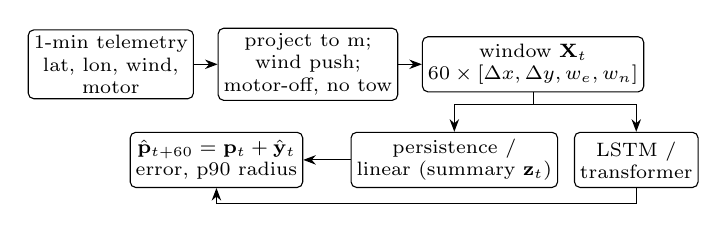
\begin{tikzpicture}[font=\scriptsize, node distance=3mm and 3mm,
  box/.style={draw, rounded corners=2pt, align=center, minimum height=7mm, inner sep=2pt},
  arr/.style={-{Stealth[length=1.6mm]}}]
\node[box] (raw) {1-min telemetry\\lat, lon, wind,\\motor};
\node[box, right=of raw] (pre) {project to m;\\wind push;\\motor-off, no tow};
\node[box, right=of pre] (win) {window $\mathbf{X}_t$\\$60\times[\Delta x,\Delta y,w_e,w_n]$};
\node[box, below=5mm of win, xshift=-10mm] (lin) {persistence /\\linear (summary $\mathbf{z}_t$)};
\node[box, right=2mm of lin] (seq) {LSTM /\\transformer};
\node[box, left=6mm of lin] (out) {$\hat{\mathbf{p}}_{t+60}=\mathbf{p}_t+\hat{\mathbf{y}}_t$\\error, p90 radius};
\draw[arr] (raw) -- (pre);
\draw[arr] (pre) -- (win);
\draw[arr] (win.south) -- ++(0,-1.5mm) -| (lin.north);
\draw[arr] (win.south) -- ++(0,-1.5mm) -| (seq.north);
\draw[arr] (lin) -- (out);
\draw[arr] (seq.south) -- ++(0,-2mm) -| (out.south);
\end{tikzpicture}
\caption{Pipeline: telemetry is projected and filtered, cut into 60-minute motor-off windows, and mapped by each model to the displacement over the next 60 minutes.}
\label{fig:pipeline}
\end{figure}

\section{Implementation}\label{sec:impl}
The code is in Python with scikit-learn and PyTorch, organised by pipeline stage: \texttt{data\_prep.py} (representation, sample selection, split, error metric; Algorithm~\ref{alg:drift} lines 1--6), \texttt{linear\_reg.py} (baselines and linear regression), \texttt{nn\_models.py} (LSTM, transformer and the shared training loop; lines 7--13) and \texttt{compare.py} (results table and chart). Every script writes to \texttt{outputs/}. The README covers the overview, installation, quick start and results; dependencies are pinned in \texttt{requirements.txt} and the data are the five 1-minute exports in the repository, so nothing needs downloading. Quick start:
{\footnotesize
\begin{verbatim}
git clone https://github.com/jakecush1/autonomous-pilot-ML
cd autonomous-pilot-ML/usv-intervention/v1_ml/rowan
python3.13 -m venv .venv && source .venv/bin/activate
pip install -r requirements.txt
python data_prep.py && python linear_reg.py
python nn_models.py lstm && python nn_models.py transformer
python compare.py
\end{verbatim}}
\textbf{Reproducibility.} Seeds for NumPy and PyTorch are fixed to 0, the split is fixed by deployment, and scaling uses training statistics only, so re-running the quick start on CPU gives the numbers in Table~\ref{tab:results} exactly; we checked this by running it twice.

\begin{table}[t]
\caption{Sanity run: endpoint error after 60 min (m) on the held-out test deployment. Full evaluation is Milestone 4.}
\label{tab:results}
\footnotesize
\begin{tabular}{@{}lccc@{}}
\toprule
Model & Median & 90th pct. & $R^2$ \\
\midrule
No drift ($\hat{\mathbf{y}}=0$) & 586 & 1515 & 0.00 \\
Persistence & 294 & 570 & 0.80 \\
Linear regression & 318 & 631 & 0.77 \\
LSTM & 247 & 497 & 0.85 \\
Transformer & \textbf{246} & \textbf{477} & \textbf{0.86} \\
\bottomrule
\end{tabular}
\end{table}

A first run (Table~\ref{tab:results}) shows the pipeline works end to end. Persistence halves the no-drift error, linear regression does not beat it on the unseen deployment, and both sequence models do, by about 16\%. Evaluation over several seeds and horizons, and turning $\hat{\mathbf{p}}_{t+H}$ into a time to boundary in the spirit of Dugan and Utne~\cite{dugan2024drifting} and an intervention probability~\cite{kristensen2022dynamic}, follow in Milestone 4. Song et al.~\cite{song2024drift} correct a physics model with a neural network; we learn drift from telemetry alone.

\bibliographystyle{ACM-Reference-Format}
\bibliography{bibliography.bib}

\end{document}
